\documentclass[conference]{IEEEtran}
\IEEEoverridecommandlockouts
\usepackage{graphicx}
\usepackage{svg}
\usepackage{amsmath,amssymb,amsfonts}
\usepackage[natbib=true, style=numeric, sorting=none]{biblatex}

\addbibresource{references.bib}

\begin{document}

\title{
    Satisfaction-modeling, the correlation to queuing duration, and
    service interruptions
}

\author{
    Hampus Avekvist \\
    \IEEEauthorblockA{
        \textit{Department of Engineering Sciences} \\
        \textit{University West}\\
        Trollhättan, Sweden \\
        hampus.avekvist@hey.com
    }
}

\maketitle

\begin{abstract}
    This article explores how queuing duration and service
    interruptions affect satisfaction from persons in a M/M/c
    queuing system. A simple model of satisfaction where queue
    duration and interruptions matter is proposed and a simulation
    using SimPy is performed. The results show that, as the number
    of services increase, so does the satisfaction. Though, the
    number of services don't meet the demand of the actors and the
    general result is a low, yet increasing, satisfaction. The
    model is simple and therefore provides several limitations that
    could inspire further work. Three levels of arrival rates are
    simulated, with the number of service desks ranging from 1 to
    100, and, unsurprisingly, the satisfaction decreases as the
    arrival rate increases. Though, all three levels converge to
    the same results as the number of service desks increase.
\end{abstract}

\begin{IEEEkeywords}
    satisfaction-modeling, service~interruptions, queue~duration
\end{IEEEkeywords}

\section{Introduction}

Waiting in turn for something is a common human experience most
have experienced. Most, if not all, have been in a line at least
once, be it the grocery checkout line, college application or
just waiting your turn at the doctors'. Alongside waiting in line,
a part of the human experience is emotional
\cite{NeuroLaunchMakingSomeoneWait} and, for this work, the change
in satisfaction from waiting in a queue. The field has previous
work, originally developed by Agner Krarup Erlang
\cite{ErlangSandsynlighedsregning} in the early 1900s when Erlang
aimed to figure out how many operators were necessary for proper
call handling in telephone exchange systems.

The paper is divided into the following parts: Section
\ref{sec:method} that proposes a simplified model of simulating
satisfaction from actors in a system based on the $M/M/c$
mathematical queuing model \cite{ChukovaUcarQueuingSystems}.
Section \ref{sec:method} also provides details on how the
simulation is performed. \ref{sec:results} show the results
following the simulation while providing an analysis of the
results and then the paper concludes with section
\ref{sec:conclusion}.

\section{Method}
\label{sec:method}

\subsection{The model}

The model is a satisfaction-oriented $M/M/c$
\cite{ChukovaUcarQueuingSystems} (see Fig.~\ref{fig:queue-diagram})
system with $c$ services, where actors start with a uniformly
distributed level of satisfaction in the range $[2,~5]$. There is
a secondary range, $[0,~5]$, for the current satisfaction of an
actor used for measurements in the simulation. The ranges are
arbitrarily chosen. Zero is the lowest level of satisfaction and
will prompt an actor to leave the system. While the actor is in
the queue, the satisfaction will decrement, alongside if they
face any difficulties using a service. 

\begin{figure}[!t]
    \centerline{
        \includesvg[width=0.3\textwidth]{figures/queue-model.svg}
    }
    \caption{
       A visual representation of what the queue can look like.
       Circles are actors, while the boxes at the top are service
       desks.
    }
    \label{fig:queue-diagram}
\end{figure}

Actors join the queue with an arrival rate of $13$ actors per $60$
minutes. If an actor faces difficulties using the service, an
arbitrary extra 30 seconds is added to the simulation time and
the actor retries. The actor retries until either the level of
satisfaction drops to zero or until they have finished using the
service. If an actor has been in the queue for at least ten
minutes, they will lose one level of satisfaction and this repeats
until they either enter a service or satisfaction reaches zero. The
actors utilize the service for a uniformly distributed simulated
time in the range $[0, 160]$ minutes. The following equation,
(\ref{eq:service-rate}), gives the service rate where $\mu$ denotes
the service rate and $c$, as above, denotes the number of services.
$80$ is the average utilization time from the previously stated
range. 

\begin{equation}
    \mu(c) = \frac{c}{80}
    \label{eq:service-rate}
\end{equation}

\subsubsection{Limitations}

The following limitations provide possible ideas for further work.

\begin{itemize}
    \item The model is limited to an unoccupied queue
        \cite{NeuroLaunchMakingSomeoneWait}.
    \item The model doesn't allow people to know how long they
        will be standing in line
        \cite{NeuroLaunchMakingSomeoneWait}.
    \item The model assumes no cultural bias
        \cite{NeuroLaunchMakingSomeoneWait}.
    \item The model is a serpentine and not a parallel queue
        \cite{NeuroLaunchMakingSomeoneWait}.
    \item Not based on real data. Data from real experiments with
        similar scenarios are required.
    \item The model only accounts for satisfaction. A person
        could e.g. be more or less patient which may affect total
        satisfaction but won't be factored in this model.
    \item The queue requires active participation to remain in
        place and is not a ``sign-up and be notified'' type of
        queue that would allow simultaneous activity.
    \item The queue is ``perpetual'' and people can come and go
        as they like. A realistic situation would be a queue tied
        to working hours that could affect customer satisfaction
        from no longer accepting requests past a certain time.
\end{itemize}

\subsection{The simulation}

The simulation software Phone Service from
\cite{AvekvistLorentzonDta400}, based on \verb|SimPy| \cite{SimPy},
codifies the model above with applied values. The number of actors
in the system is hard-coded to $800$, arbitrarily chosen, alongside
three arrival rates, $\lambda~\in~\{3,~13,~23\}$, actors joining
the system per $60$ minutes. This is accomplished in three separate
simulation runs. The simulation generates data that is saved in a
\verb|SQLite3| \cite{SQLite3} database file that a secondary
program in the same module, called \verb|database_reader.py|, uses
to perform calculations and generate graphs. The simulation
software speaks in terms of phones and phone booths but the
simulation is more generalized so it may be used to simulate
general satisfaction-based systems where actors leave after
interruptions.

The data that is saved from the simulation is firstly the
satisfaction at the start of the simulation for every actor, paired
with the number of services available for the simulation
\cite{AvekvistLorentzonDta400}. Secondly, the service- and arrival
rates are stored and lastly the end result of the simulation is
saved. The end results contain the queue size upon an actor's
arrival in the queue, the queue duration and satisfaction for said
actor, alongside the number of services for this simulation. The
data is used by \verb|database_reader.py| to calculate averages and
generate the graphs provided in section \ref{sec:results}.

\section{Results}
\label{sec:results}

The results are provided from running the simulations ten times
for each $c$ and $\forall~c~\in~[1,~100]$, $c~\in~\mathbb{N}$. This
is to reduce the bias from the random number generator. These are
also run three times, one for every aforementioned $\lambda$.

Firstly, as the number of services increase linearly, so does the
service rate. This follows from (\ref{eq:service-rate}).
Furthermore, the queue time is reduced in an initially quick manner
but as the number of services reach ten, the queue time is
stabilized shown by Fig.~\ref{fig:queue-time-3}. Lastly, the
satisfaction increases in a similar, but opposite direction, from
the queue time, as shown in Fig.~\ref{fig:satisfaction-3}.

\begin{figure}[htbp]
    \centerline{
        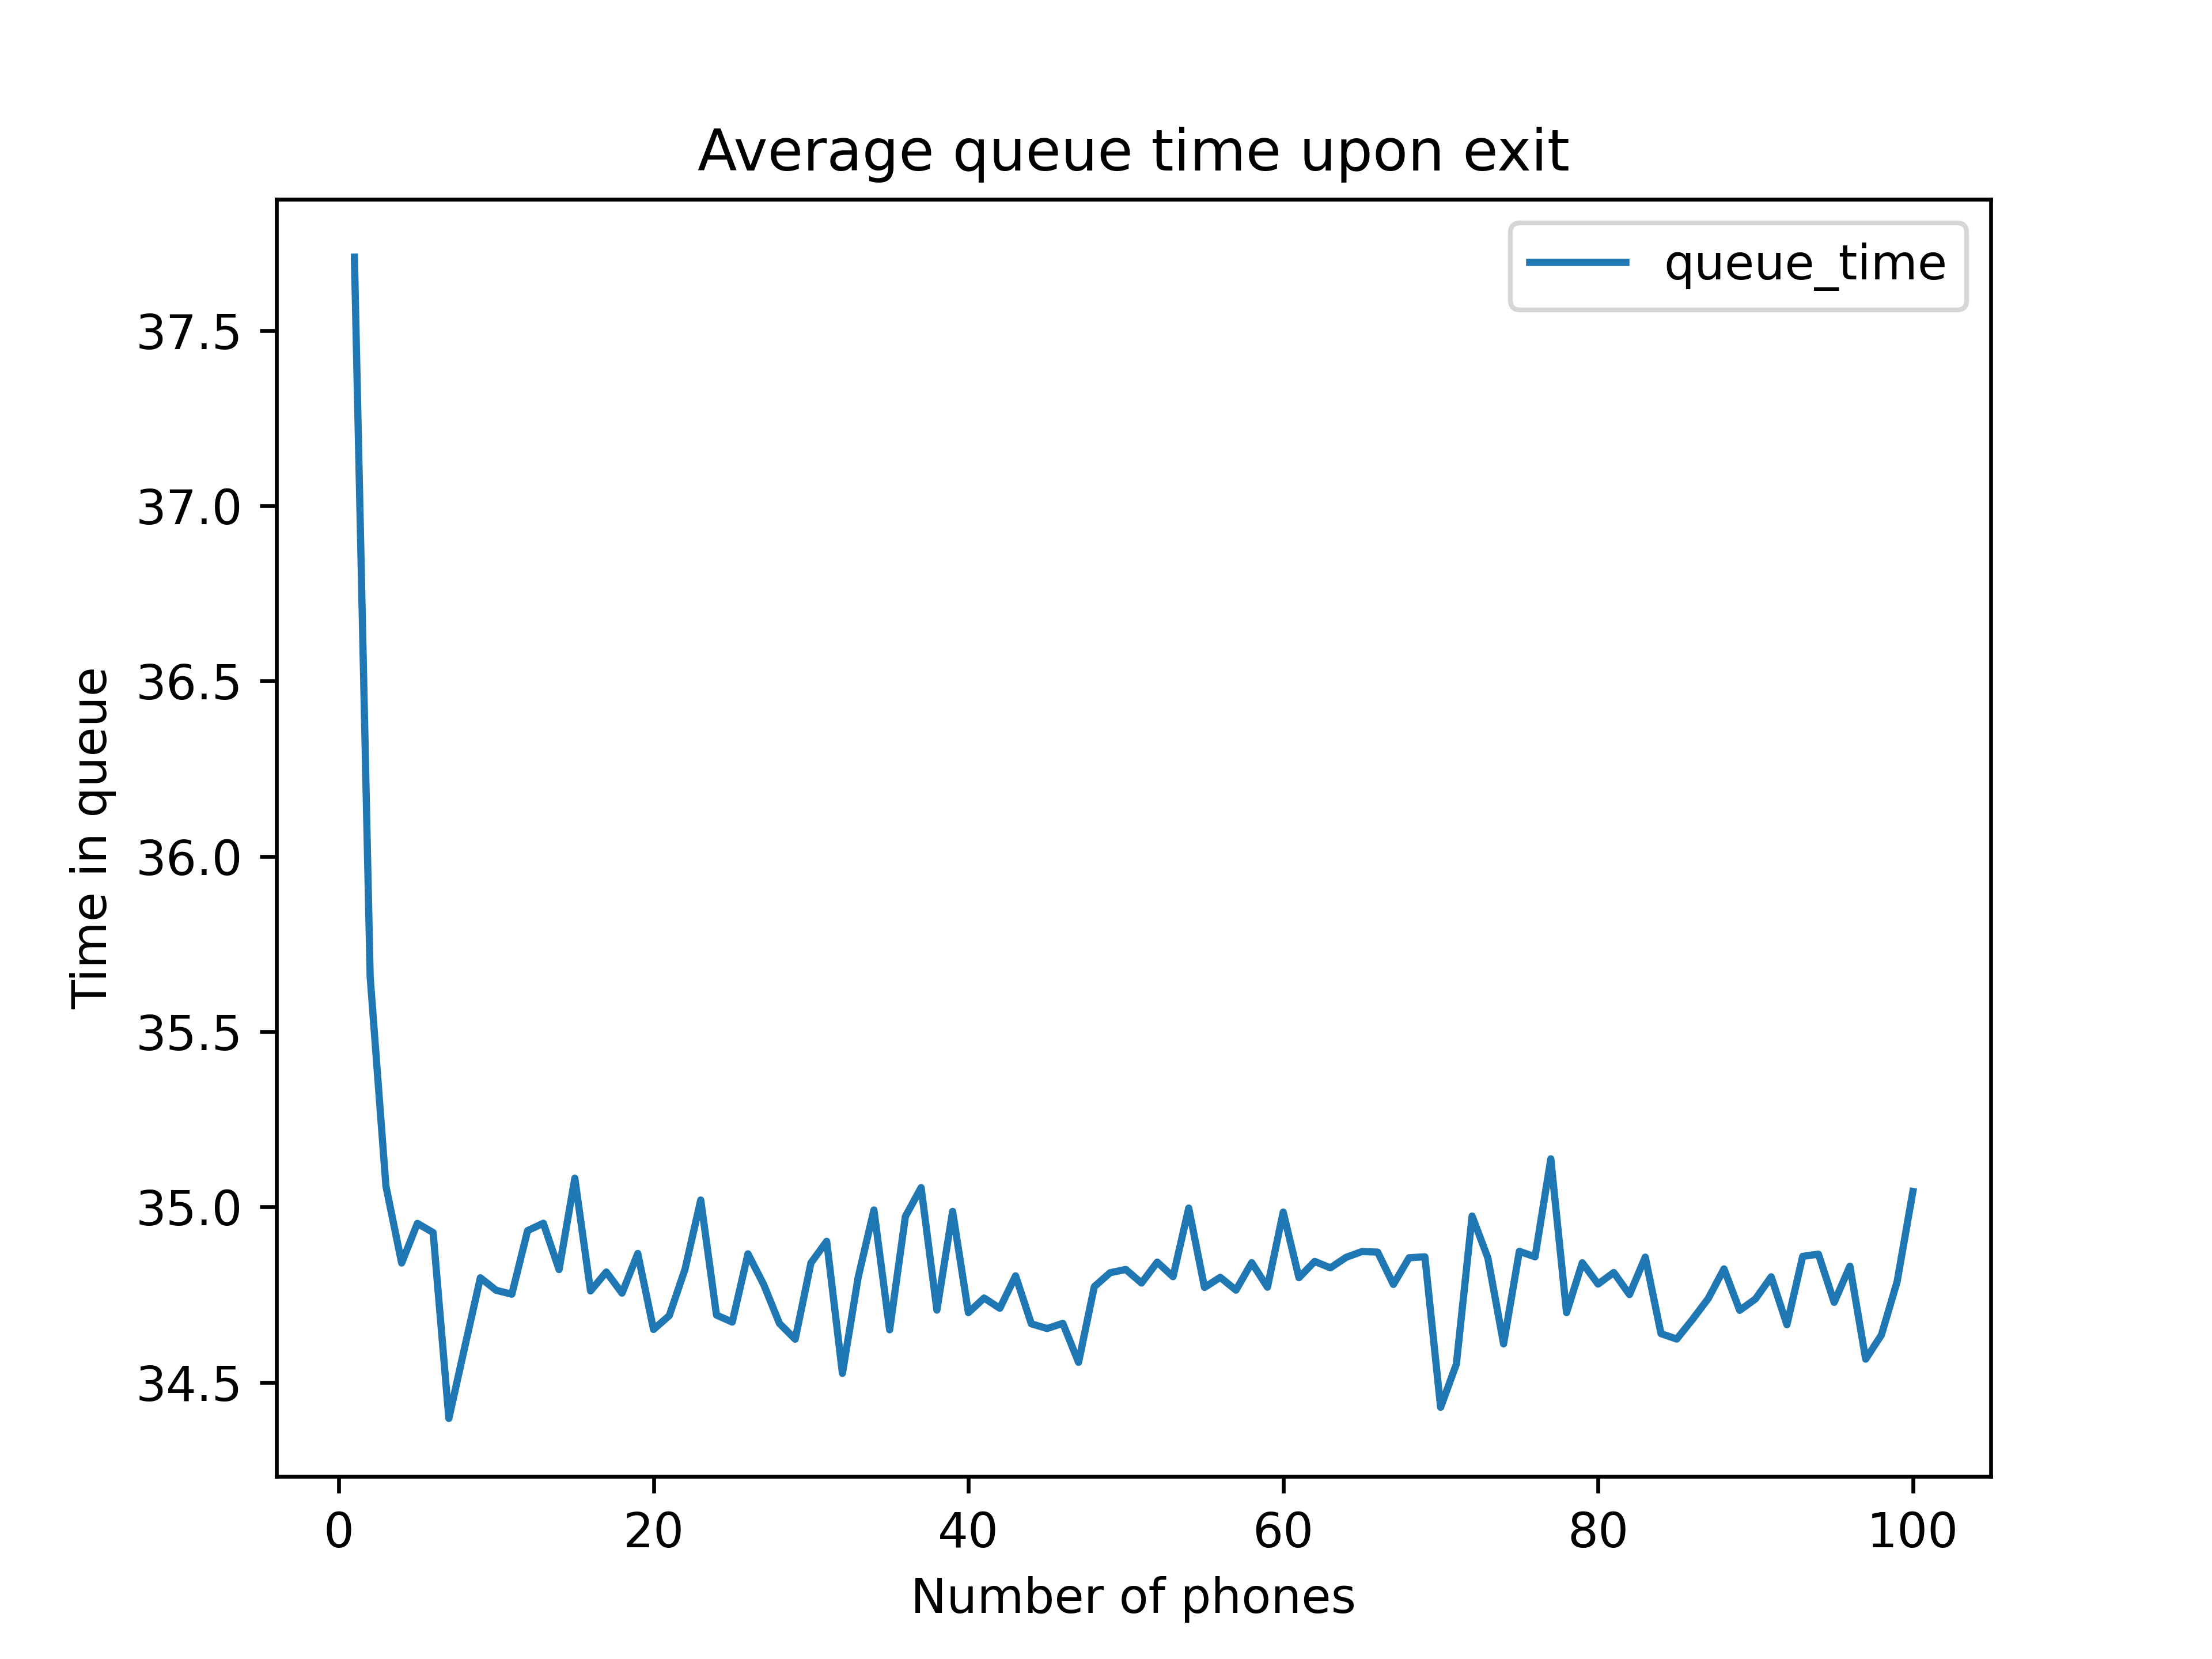
\includegraphics[width=0.4\textwidth]{
            figures/queue-time-3.png
        }
    }
    \caption{
        The average time spent in line based on the number of
        phones (services) when $\lambda = 3$
    }
    \label{fig:queue-time-3}
\end{figure}

\begin{figure}[htbp]
    \centerline{
        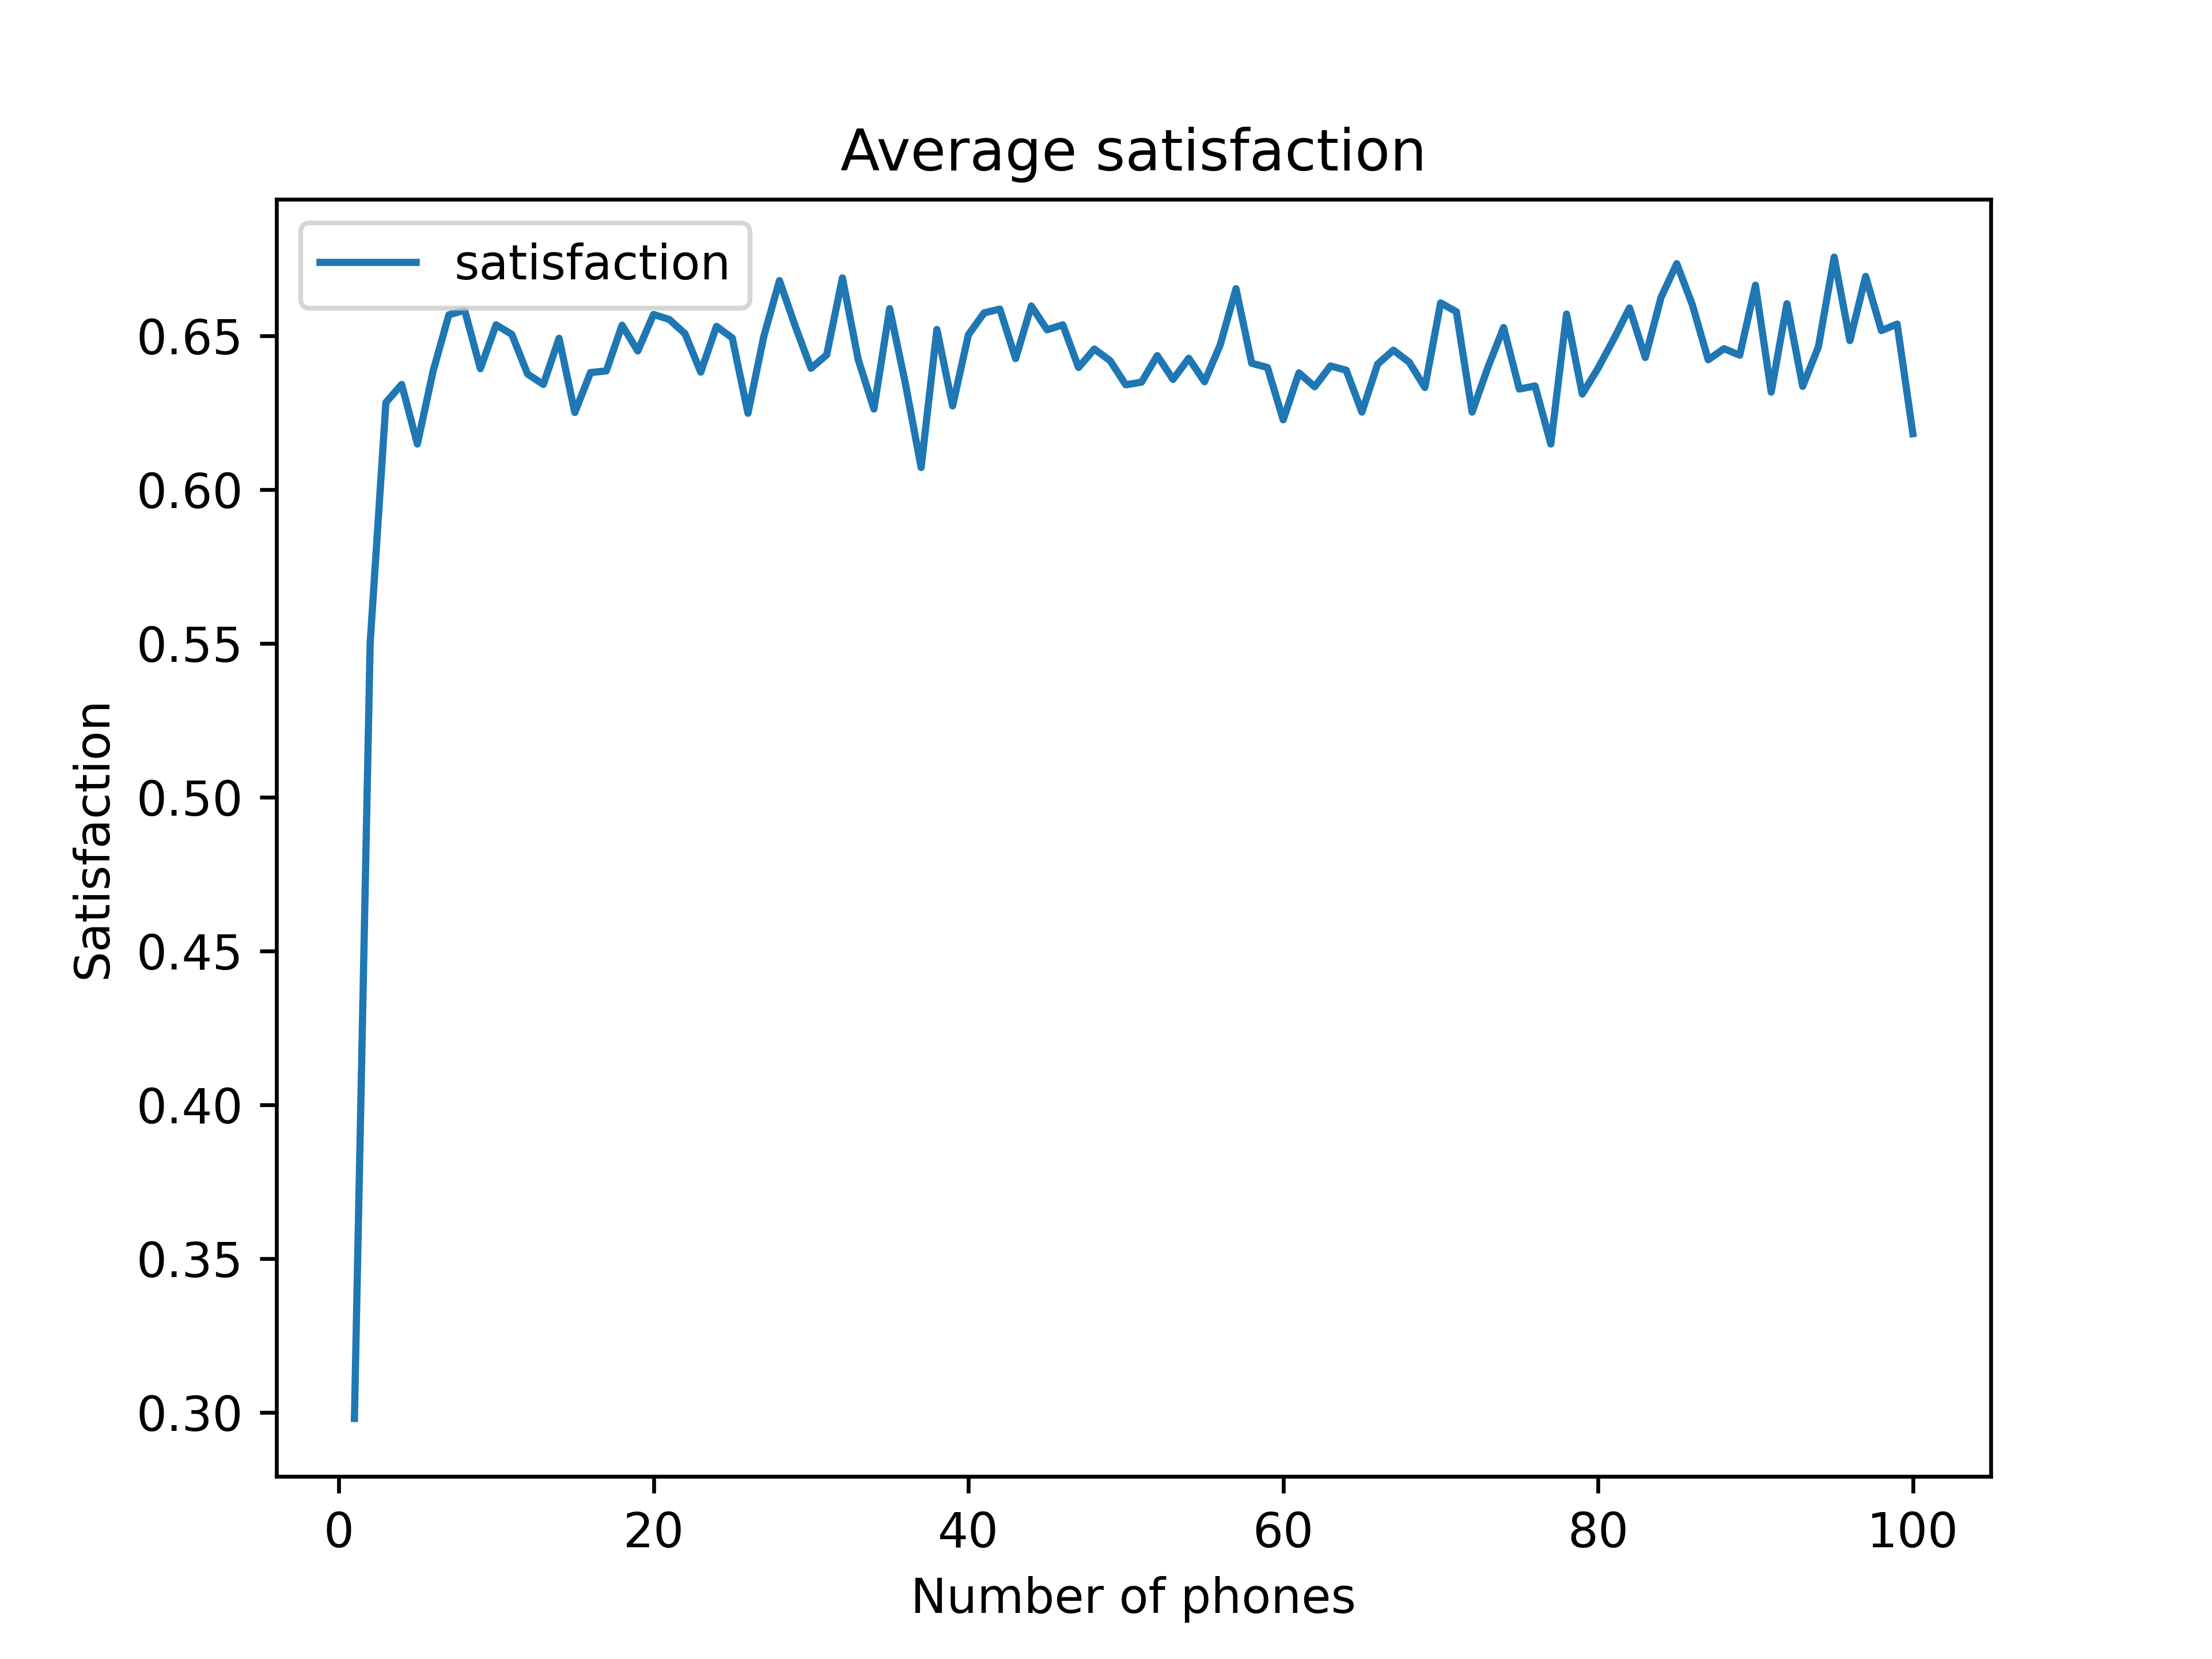
\includegraphics[width=0.4\textwidth]{
            figures/satisfaction-3.png
        }
    }
    \caption{
        The average level of satisfaction based on the number of
        phones (services) when $\lambda = 3$
    }
    \label{fig:satisfaction-3}
\end{figure}

As the number of services increase, so does the satisfaction. This
is not unexpected, as more actors can be served at the same time,
which also decreases the time in line. Though, as
Fig.~\ref{fig:satisfaction-3} suggests, most actors are
either entirely dissatisfied having reached zero, or very
dissatisfied, on the brink of leaving the system. This is shown by
the left side of Fig.~\ref{fig:queue-time-3} as actors, on average,
remain in the system between $34$ and $38$ minutes. Since an actor
loses a level of satisfaction per ten minutes spent in queue, they
lose three levels of satisfaction simply by remaining in line. If a
service interruption occurs at this point, it's highly probable
that the actor will leave the system. The starting level of
satisfaction is uniformly distributed in the range of $[2,~5]$,
meaning a majority of actors will leave the system. Though, as
actors leave the system, other actors receive a reduced waiting
time, leading to the spikes in the graph.

Fig.~\ref{fig:satisfaction-3} and Fig.~\ref{fig:queue-time-3} only
display the simulation when $\lambda = 3$. As $\lambda$ changes to
the remaining two elements the results in
Fig.~{fig:satisfaction-13}, Fig.~{fig:queue-time-13},
Fig.~{fig:satisfaction-23} and Fig.~{fig:queue-time-23} are
procured that demonstrate a reduced satisfaction and increased
queue time, especially when $\lambda = 23$. This is unexpected as
more actors joining the system should affect the queue time, which,
in turn affects the satisfaction. The main difference is not an
increased queue duration and satisfaction, but rather how many
services are required to reach the same level of waiting time and
satisfaction. All results approach a satisfaction level near $0.65$
and queue time near $34.5$, but when $\lambda = 13$ it requires
ten services and when $\lambda = 23$ it requires $20$ services.

\begin{figure}[htbp]
    \centerline{
        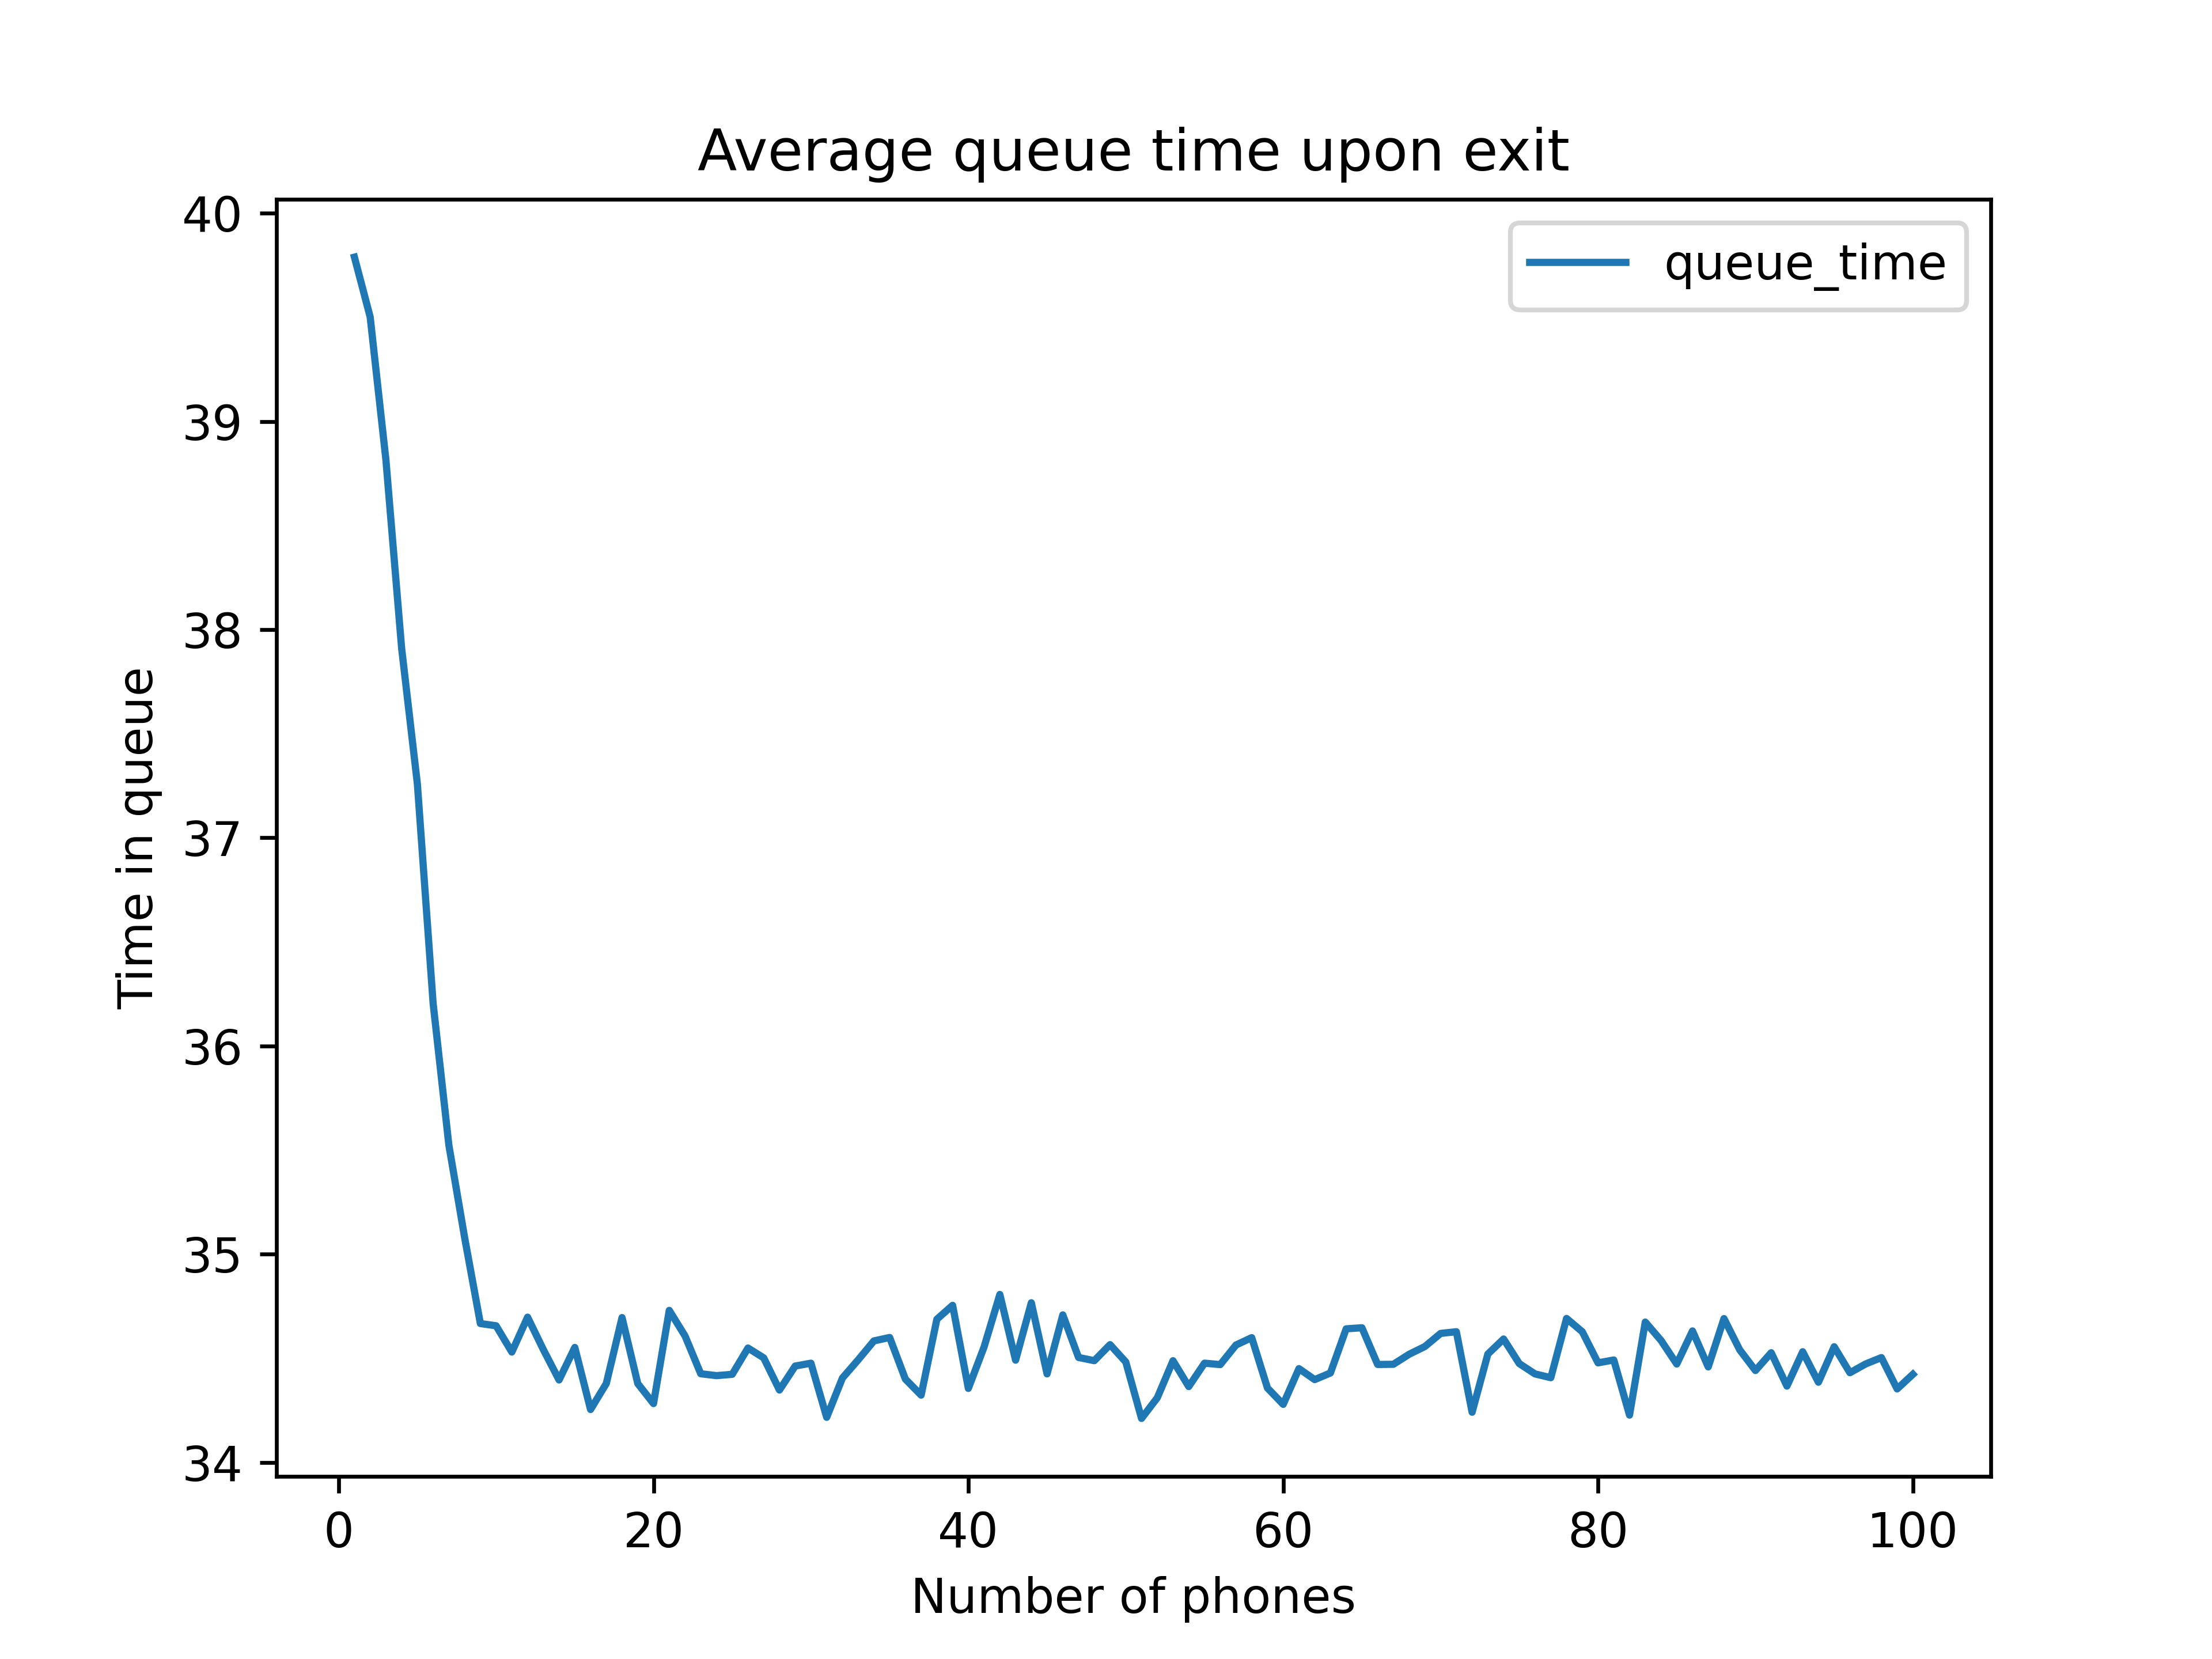
\includegraphics[width=0.4\textwidth]{
            figures/queue-time-13.png
        }
    }
    \caption{
        The average time spent in line based on the number of
        phones (services) when $\lambda = 13$
    }
    \label{fig:queue-time-13}
\end{figure}

\begin{figure}[htbp]
    \centerline{
        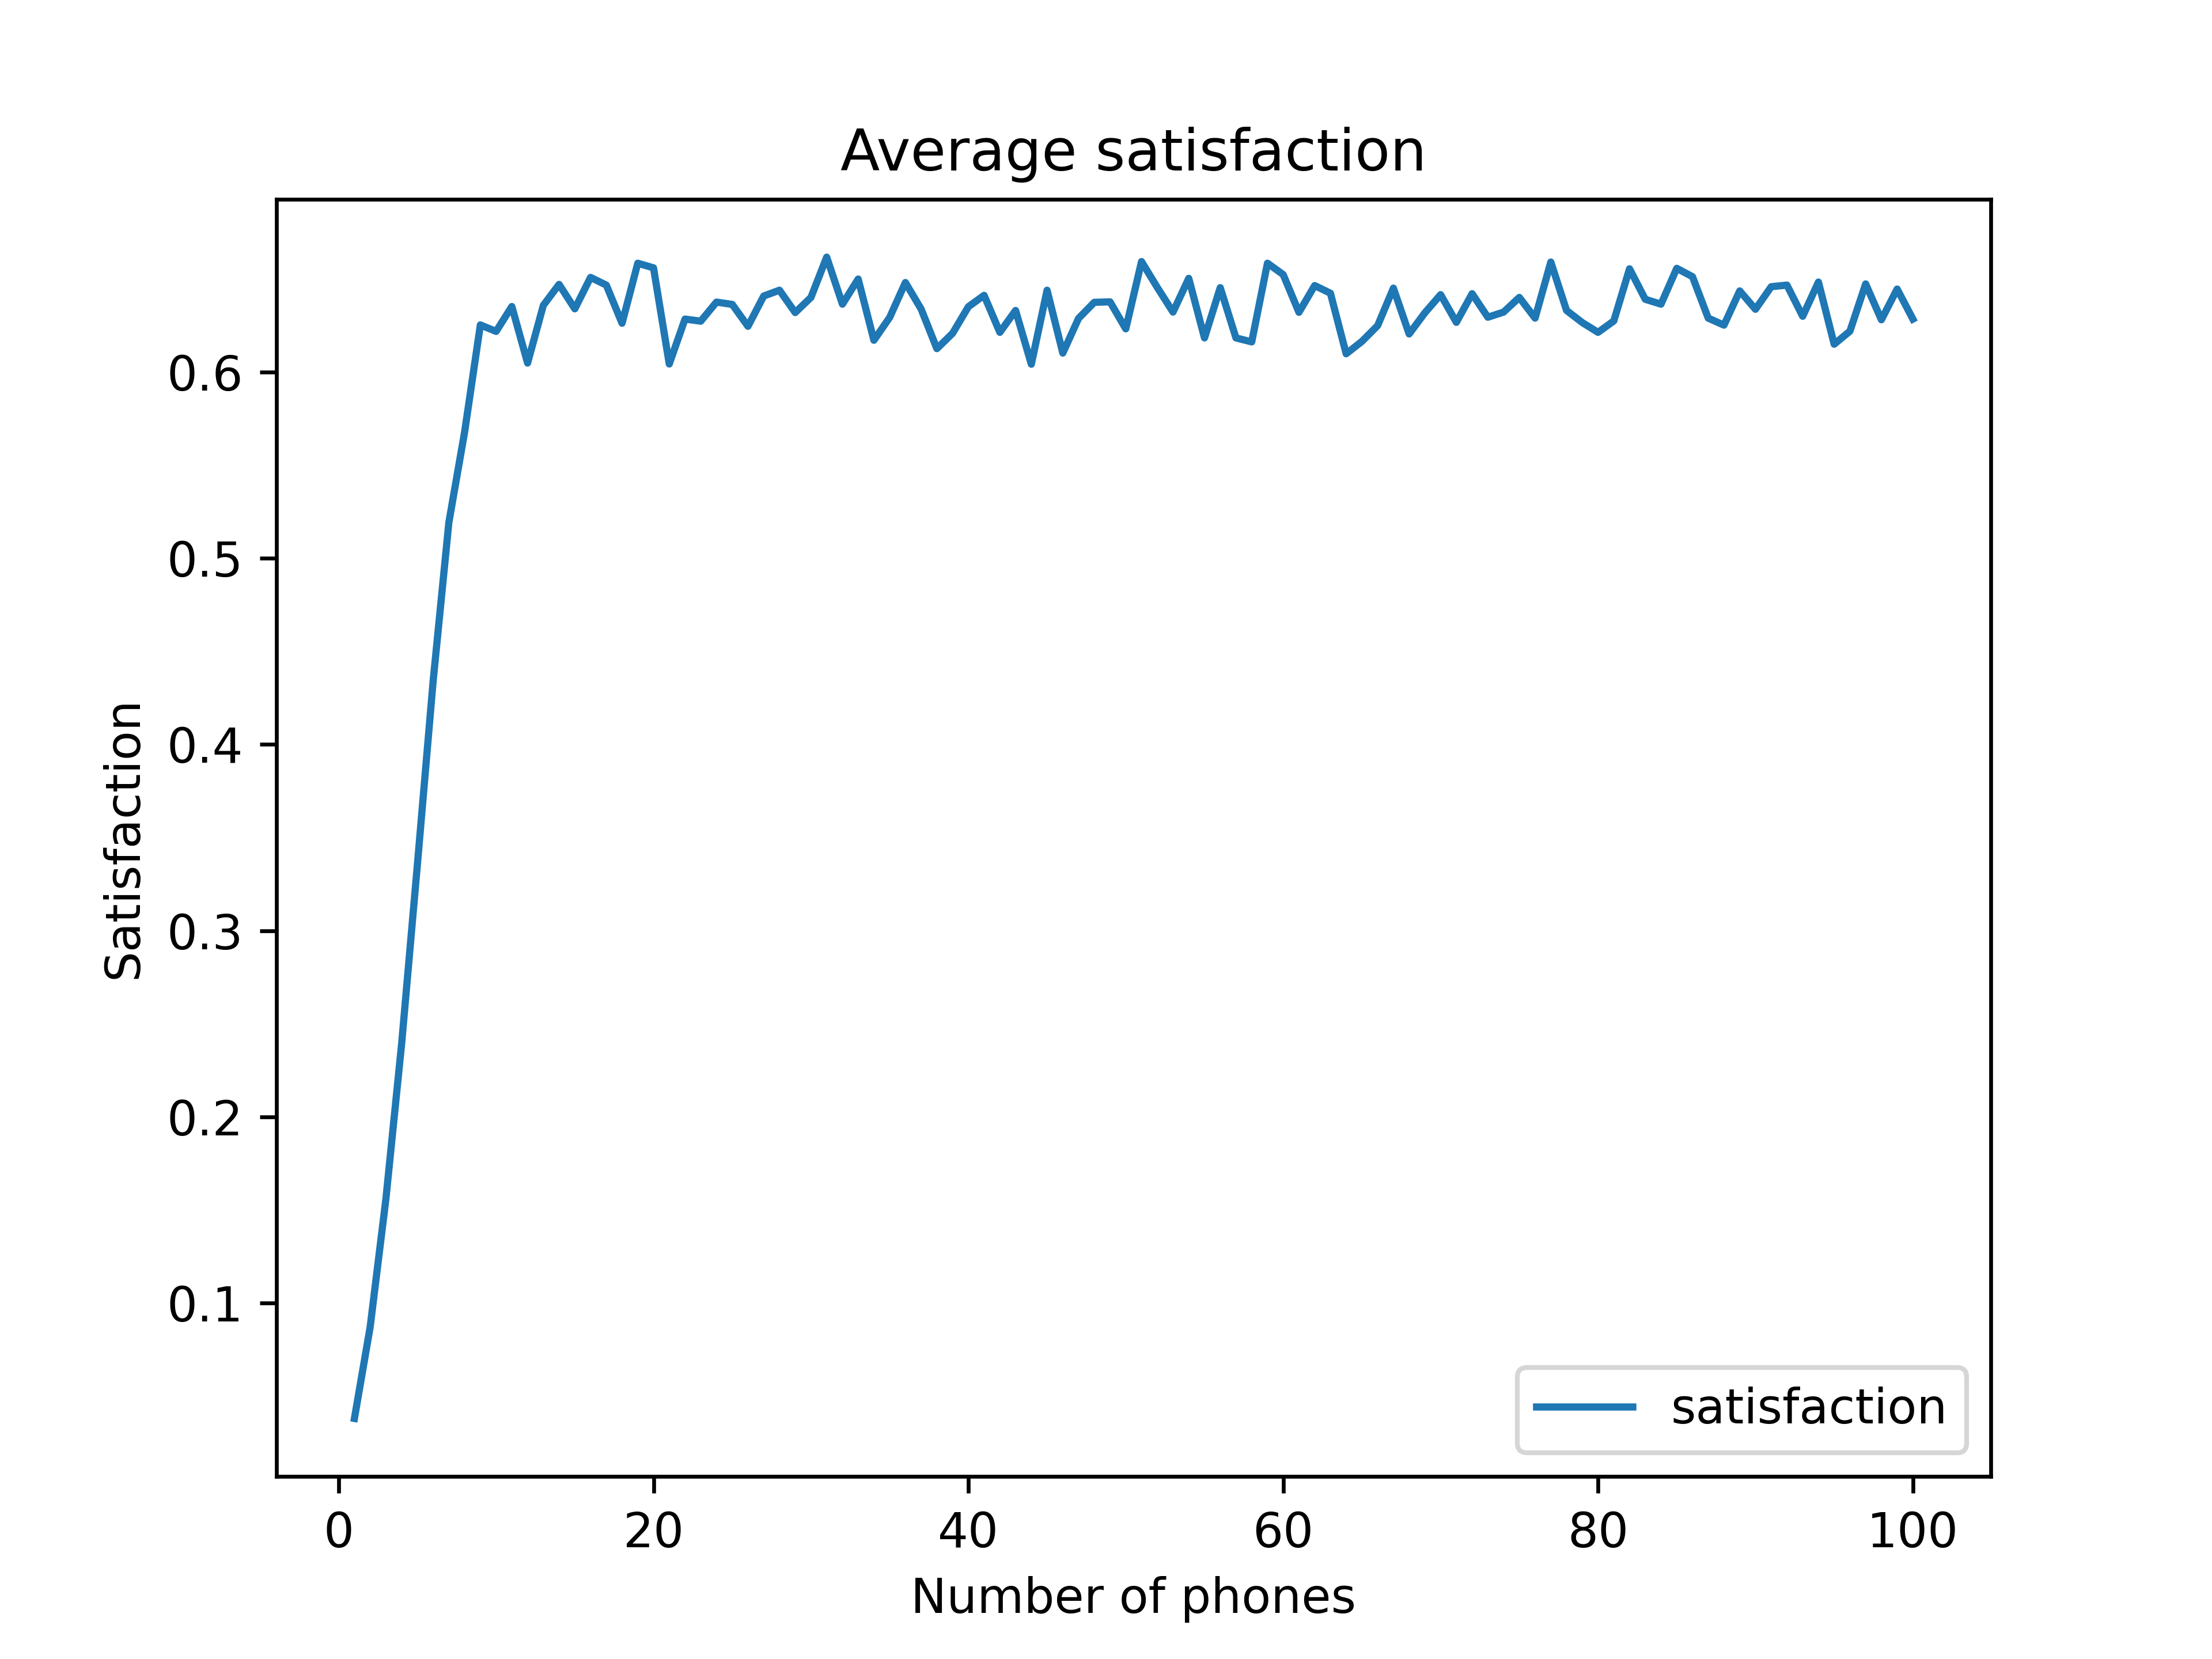
\includegraphics[width=0.4\textwidth]{
            figures/satisfaction-13.png
        }
    }
    \caption{
        The average level of satisfaction based on the number of
        phones (services) when $\lambda = 13$
    }
    \label{fig:satisfaction-13}
\end{figure}

\begin{figure}[htbp]
    \centerline{
        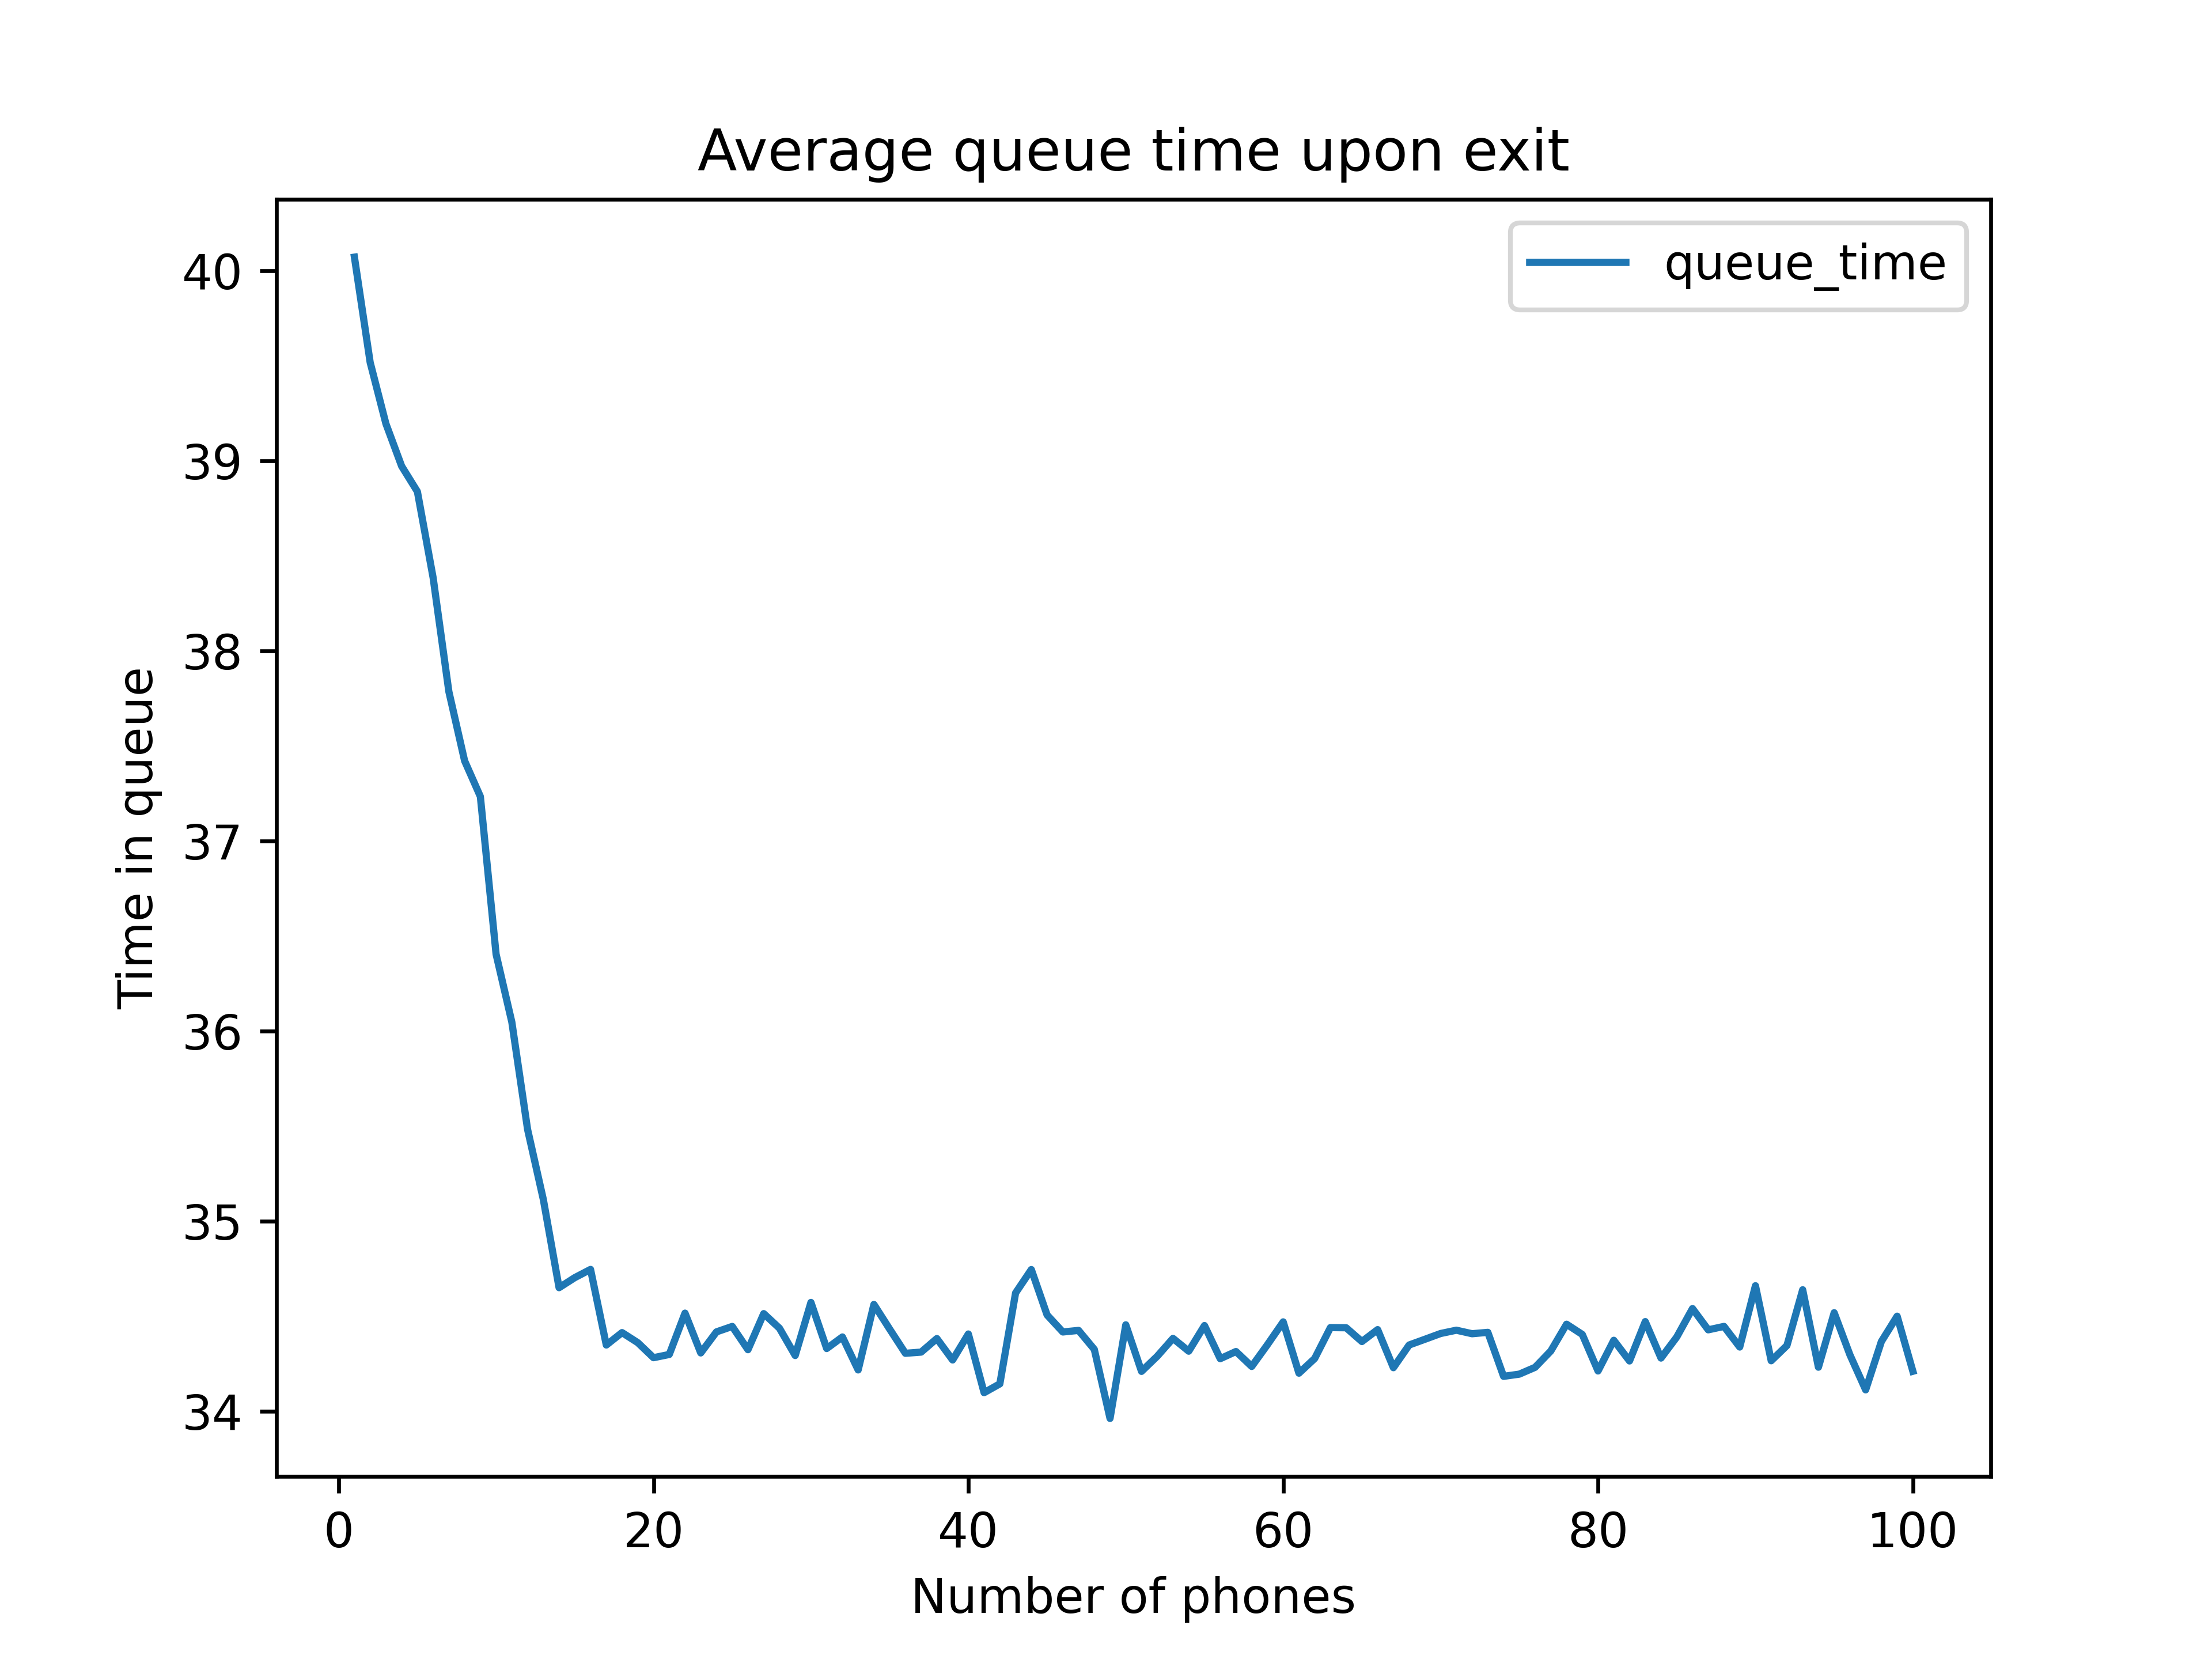
\includegraphics[width=0.4\textwidth]{
            figures/queue-time-23.png
        }
    }
    \caption{
        The average time spent in line based on the number of
        phones (services) when $\lambda = 23$
    }
    \label{fig:queue-time-23}
\end{figure}

\begin{figure}[htbp]
    \centerline{
        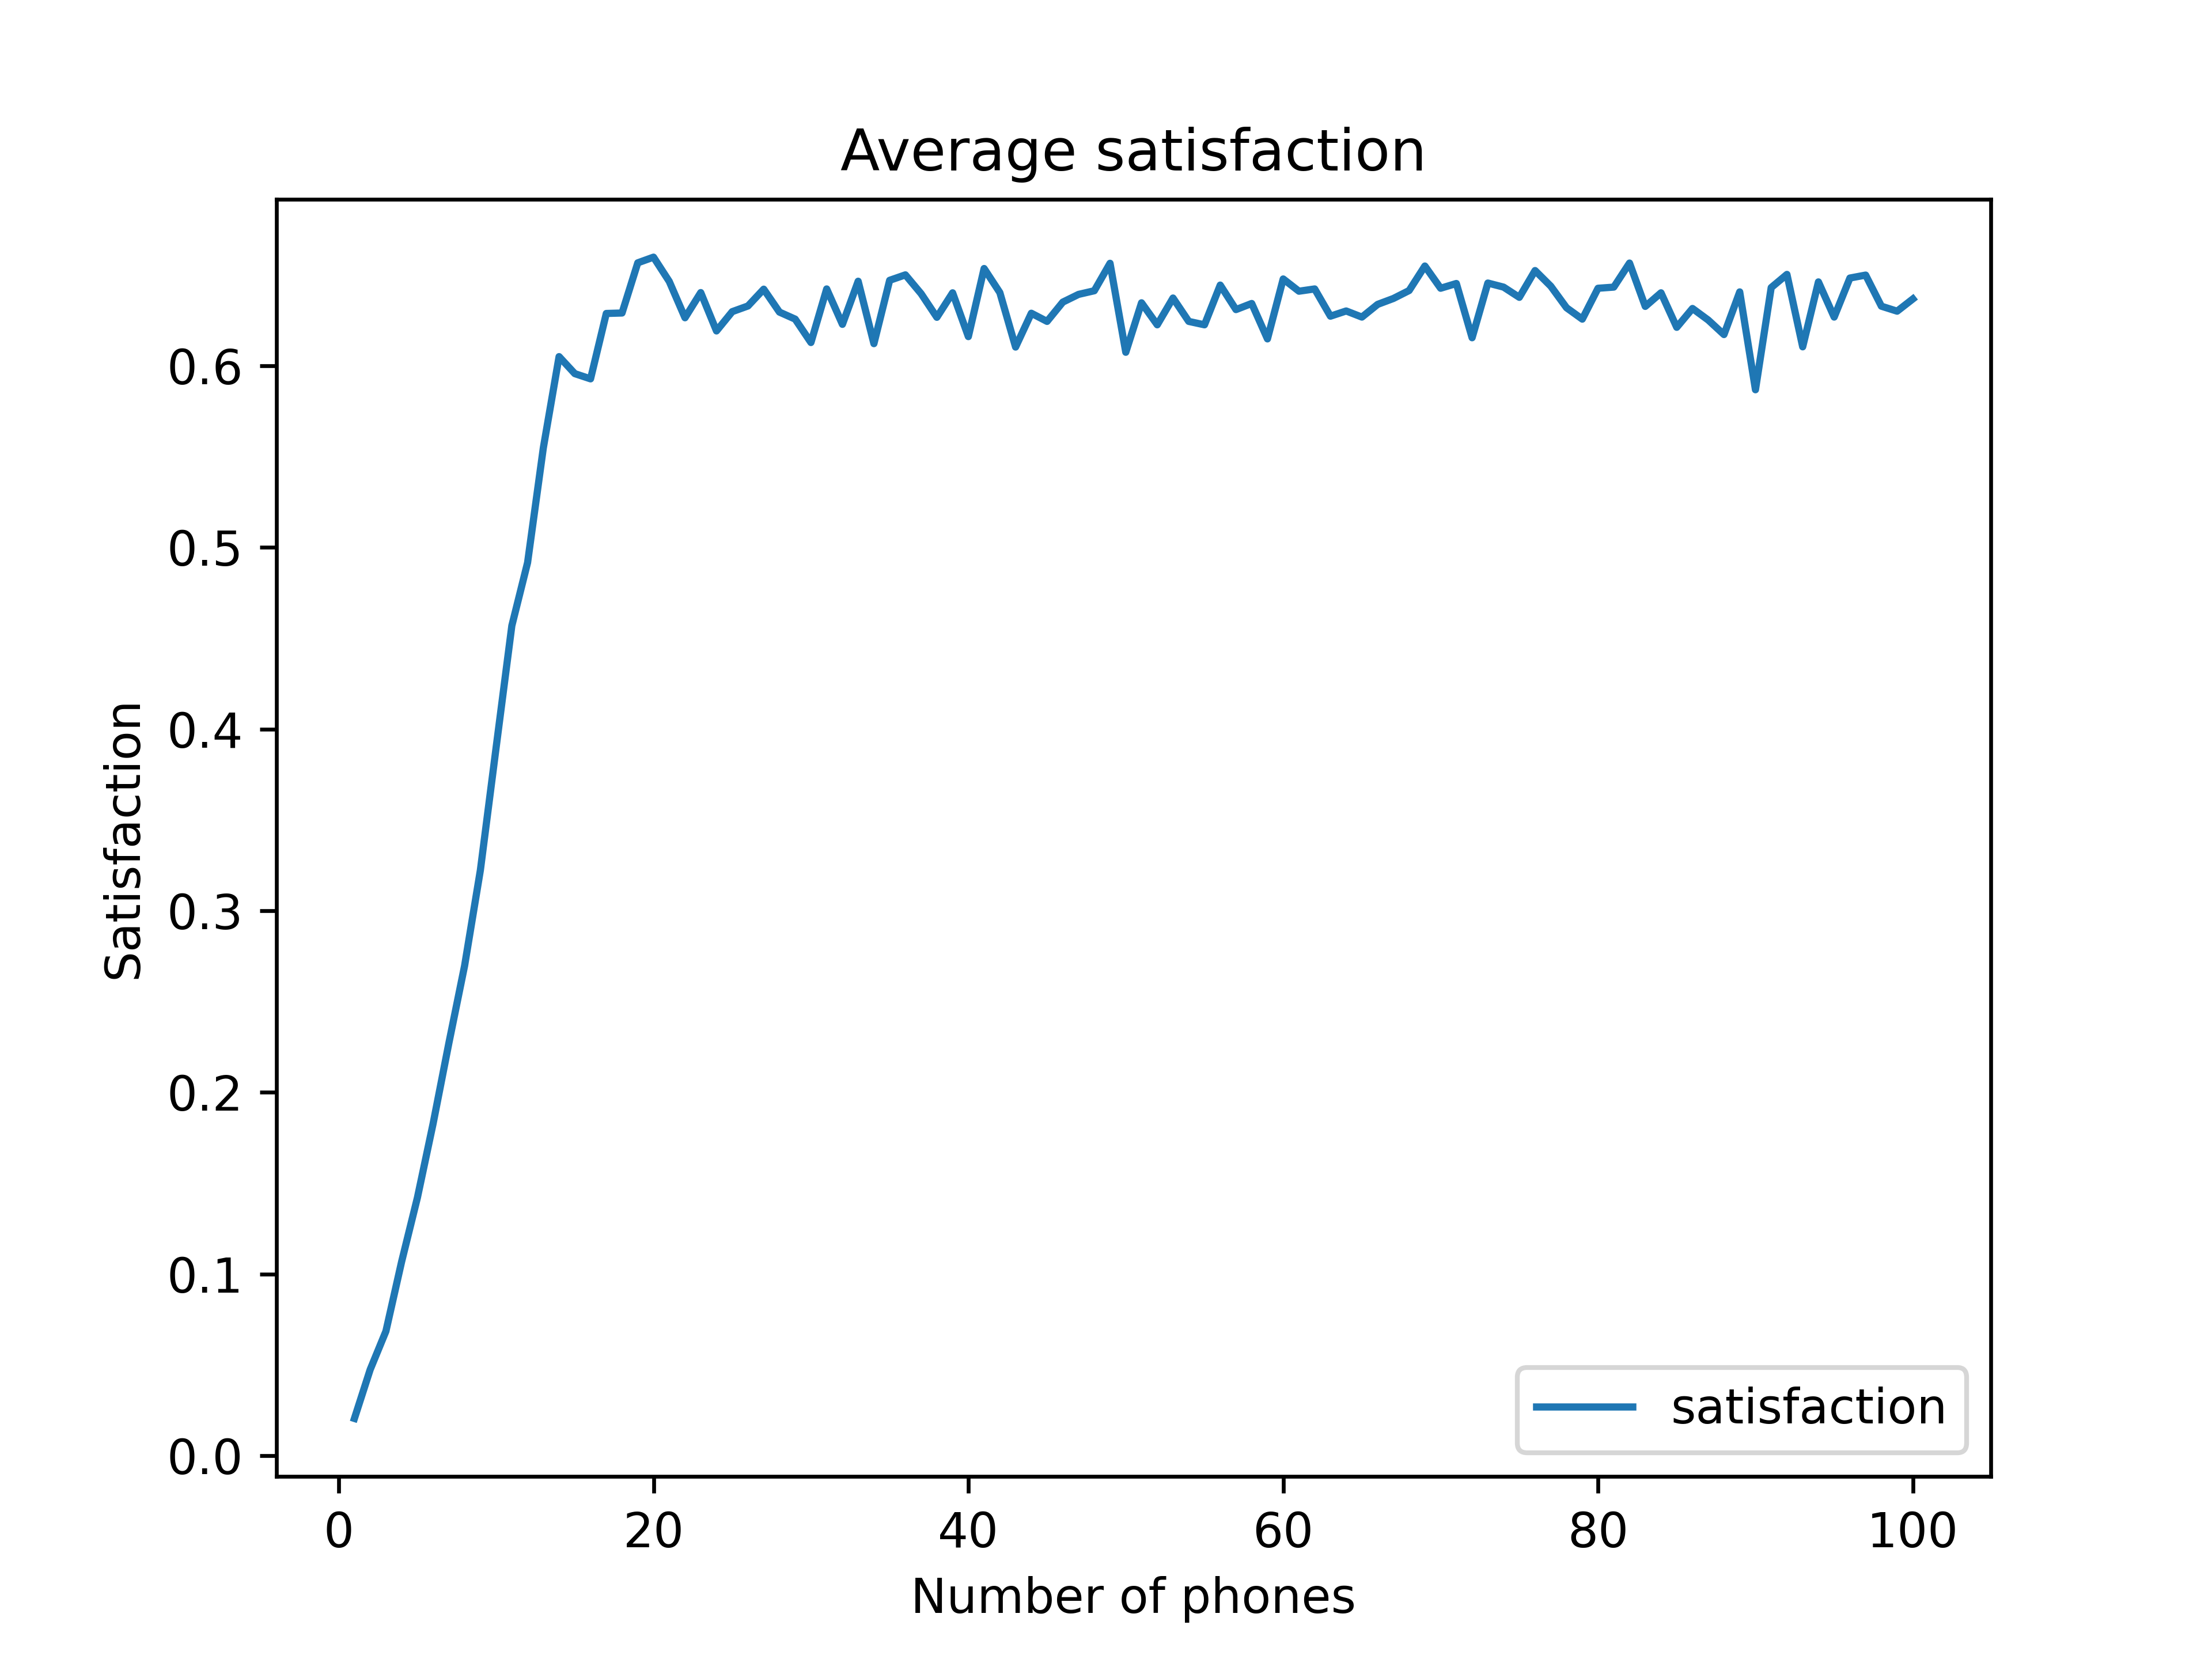
\includegraphics[width=0.4\textwidth]{
            figures/satisfaction-23.png
        }
    }
    \caption{
        The average level of satisfaction based on the number of
        phones (services) when $\lambda = 23$
    }
    \label{fig:satisfaction-23}
\end{figure}

\section{Conclusion}
\label{sec:conclusion}

The satisfaction increases as the queue time is reduced, which
depends on how many services that are available in the system. As
the arrival rate changes, so does the required number of services
to accommodate the increasing number of actors.

\section*{Acknowledgment}
\label{sec:acknowledgment}

I'd like to thank Felicia Lorentzon for the assistance and ideas
when working on the simulation, as well as the zany jokes we've
made along the way to keep us sane during the long hours. I'd also
like to thank Rashid Ali for his assistance when we had questions
and problems with our simulation and when we wanted to change our
model.

\printbibliography

\end{document}
